%% ===================================================================
%% PART I
%% ===================================================================
\part{Foundations}

%% -------------------------------------------------------------------
\section{Introduction: the geometry of non-embedding}\label{sec:intro}

\subsection{Relation to arithmetic occurrence geometry}\label{sec:aog}

This paper continues the study of \emph{arithmetic occurrence geometry}, a term defined in the companion planar manuscript \cite{PaperA} (in its Introduction and, formally, directly after the derivation of the occurrence fibre $F_x$ in its Section~2): the study of finite arithmetic occurrence fibres, their exact coordinate relationships, and explicitly specified geometric realizations constructed upon those relationships. The occurrence coordinates are determined by arithmetic; the cell constructions are separately specified structures, so that the intrinsic organization of the occurrences is distinguished from the properties of a particular realization. Whereas the companion manuscript investigates exceptional topology and convex stabilization for two active prime coordinates, the present paper addresses embedding obstructions in a specified higher-dimensional \emph{binary $0/1$ Graver-cell construction}.

\emph{Specialization.} In the notation of this paper, the arithmetic occurrence fibre is replaced by the fibre $F=C\setminus\{0\}$ of a binary code $C=\ker M$ (the nonzero $0/1$ points of the relation lattice $\Lambda_M$), and the realization is the Graver-cell construction of Section~\ref{sec:cells} restricted to the box $[0,1]^n$. Binary relation lattices form a mathematically tractable family in which circuit decompositions, cell collisions and minimum obstruction ranks can be investigated exactly. The conclusions concern this specified construction. They do not presume that every binary configuration is realized by a rational occurrence fibre (see also Section~\ref{sec:intro-scope}). We use \emph{arithmetic occurrence geometry} in the sense defined in the companion manuscript \cite{PaperA}: the study of distinct arithmetic occurrence fibres, their exact coordinate relationships, and explicitly specified geometric realizations. The present paper investigates a higher-dimensional binary $0/1$ specialization of the Graver-cell construction. The binary model is defined for arbitrary binary codes; its conclusions apply to actual UNNS occurrence fibres whenever the required arithmetic realization is established. The term is used as in the companion manuscript, as a defined term of this research programme; it is not a claim to belong to, or to inherit the definitions of, the established field of arithmetic geometry.

\subsection{The question}

A binary matrix $M\in\F_2^{m\times n}$ defines a lattice
\[
\Lambda_M=\{\alpha\in\Z^n:\ M\alpha\equiv 0 \pmod 2\},
\]
and the integer points of the unit box $[0,1]^n$ in $\Lambda_M$, with the origin deleted, form a finite set $F$, the \emph{fibre}. Identifying a $0/1$ vector with a word of $\F_2^n$, the fibre is the set of nonzero words of the binary code $C=\ker M$. Inside this lattice there is a canonical family of lattice vectors, the \emph{Graver basis}: the conformally minimal nonzero elements of $\Lambda_M$. A \emph{cell} is a parallelepiped spanned by linearly independent Graver vectors all of whose corners lie in $F$. The union of all cells is a geometric object assembled from the fibre in a way that depends on nothing but the lattice.

The question of this paper is the following. \emph{When do the cells of the box fit together as a polyhedral complex, meeting only in common faces?} We call the box \emph{embedded} when they do, and \emph{non-embedded} when two distinct cells have intersecting relative interiors. In the latter case the pair is a \emph{collision}. The smallest affine space containing a collision is its \emph{witness space}, and the least dimension of such a space is the \emph{minimum witness rank} $\rmin$ of the box.

The motivation comes from the arithmetic of occurrences in the UNNS nest recursion, where relation lattices of precisely this congruence type arise and where the cells describe which exponent vectors are connected by minimal moves \cite{PaperA,GEOIv001,GEOIv002,GEOIv003}. Nothing below depends on the arithmetic origin. The frozen model used here is purely combinatorial: it consists of the lattice $\Lambda_M$, its Graver basis, the box $[0,1]^n$, and the cells defined above. All objects are defined in Sections~\ref{sec:binary}--\ref{sec:cells}, and every statement is proved from those definitions.

\subsection{A first picture}

The smallest non-embedded box has $n=4$ and $C=E_4$, the even-weight code of length~$4$ (a single parity check $M=(1\,1\,1\,1)$). Its fibre is the seven nonzero even words: the six words of weight two and the word $1111$. The six weight-two words are the vertices of a regular octahedron in the affine hyperplane $\sum x_i=2$ of $\R^4$. Three of the cells are the three \emph{equatorial squares} of that octahedron, spanned by pairs of disjoint two-element supports: $\{12,34\}$, $\{13,24\}$, $\{14,23\}$. Any two of the three squares share a diagonal and all three contain the centre $(\frac12,\frac12,\frac12,\frac12)$ in their relative interiors. The three squares do not meet in common faces, so the box is non-embedded, and any two of them span only a $3$-dimensional affine space; see Figure~\ref{fig:rank3} and Section~\ref{sec:E4}.

The purpose of this paper is to show that this picture is universal. Every non-embedded box of the frozen binary model, whatever its length $n$ and nullity $k=\dim C$, contains a collision that is as small as that one: two cells spanning an affine space of dimension \emph{exactly three}, and none spans fewer. The proof goes through a rigid combinatorial structure on the circuits of minimal non-embedded boxes: a vector-space partition of $\F_2^{k-1}$ and two quadratic identities that force many two-circuit partitions of the all-ones word.

\subsection{Main results}

Throughout, a \emph{box} is a binary code $C\le\F_2^n$ (Definition~\ref{def:box}); circuits are minimal supports of nonzero words; a box is \emph{minimal} if it is non-embedded but every box obtained by deleting one coordinate (shortening) is embedded. The following statements are proved in this paper. The numbering of the corresponding source theorems in the GEO-I series is given in Appendix~\ref{app:crosswalk}.

\begin{description}
\item[Theorem A (circuit-partition criterion; \cref{thm:E1}).] A box is non-embedded if and only if some set of coordinates has two distinct partitions into circuits; equivalently, some codeword has two distinct decompositions into disjoint circuits.

\item[Theorem B (structure of minimal boxes; \cref{thm:F1,thm:rigid,thm:affine}).] In a minimal non-embedded box the all-ones word $\one$ lies in the code, no circuit is a single coordinate, every codeword other than $0$ and $\one$ has a \emph{unique} decomposition into disjoint circuits, and, after identifying coordinates that agree on every codeword, the box is a spanning subset $X$ of the affine space $\AG(k-1,2)$ with $|X|=p\ge k+1$. Isomorphism classes correspond to $\AGL(k-1,2)$-orbits of such subsets.

\item[Theorem C (vector-space partition; \cref{thm:vsp,thm:counting,thm:parseval}).] The partitions $P$ of $\one$ into circuits, with $m_P$ blocks, give subspaces $V_P\le C$ of dimension $m_P$ whose images in $C/\langle\one\rangle\cong\F_2^{k-1}$ partition the nonzero vectors, so that
\[
\sum_P\bigl(2^{m_P}-2\bigr)=2^k-2,\qquad
\sum_P\bigl(2^{m_P}S_P-2p^2\bigr)=p\,(2^k-2p),
\]
where $S_P$ is the sum of the squared block sizes.

\item[Theorem D (many two-block partitions; \cref{thm:L6,thm:W2}).] If $p\ge9$ the number $n_2$ of partitions of $\one$ into exactly two circuits satisfies $n_2\ge p-1$, with equality for $p\ge10$ only for $X=\AG(k-1,2)$. For $p\le 8$ a finite check shows $n_2\ge3$. Hence every minimal non-embedded box has $n_2\ge2$ (condition W2).

\item[Theorem E (universal rank three; \cref{thm:rank3}).] Every non-embedded box of the frozen binary model has $\rmin=3$. In particular no minimal non-embedded box has minimum witness rank $4$ or more.
\end{description}

Section~\ref{sec:E4} gives the explicit rank-three obstruction for $E_4$ together with infinite families (Reed--Muller supports $\AG(k-1,2)$), and Section~\ref{sec:classify} reports the exact classification of minimal reduced boxes for $k=3,4,5,6$ ($1$, $3$, $12$ and $215$ classes). The classification is \emph{not} used in the proof of Theorem E.

\subsection{Proof architecture}

The logical dependencies are summarised in Figure~\ref{fig:deps}. The route is:
\[
\text{Thm~A}\ \Rightarrow\ \text{Thm~B (full support, rigidity, affine reduction)}\ \Rightarrow\ \text{Thm~C}\ \Rightarrow\ \text{Thm~D}\ \Rightarrow\ \text{Thm~E}.
\]
The last step is the combination of three ingredients: a local construction showing that two distinct two-circuit decompositions of one word produce a collision of rank three; a general lower bound, valid for \emph{every} collision, showing rank three is the least possible; and a reduction showing that every non-embedded box contains a minimal one by shortening, with collisions lifting to the larger box without changing their rank.

\subsection{Scope and non-claims}\label{sec:intro-scope}

\begin{enumerate}
\item \emph{Frozen model.} All results concern the frozen binary $0/1$ Graver-cell model defined in Section~\ref{sec:binary}: the box $[0,1]^n$ of the lattice $\Lambda_M$ over $\F_2$. Other moduli, alphabets, larger boxes $Q>\one$ or non-binary lattices are not treated (Section~\ref{sec:open}).
\item \emph{Realizability.} The model contains a cell structure for \emph{every} binary code $C$. The paper does \textbf{not} claim that every binary code arises from a rational arithmetic occurrence fibre, nor that any particular code does. The relation of the model to arithmetic is discussed only in the companion manuscript \cite{PaperA} and the cited releases.
\item \emph{Meaning of $\rmin$.} The number $\rmin$ is the \emph{minimum} over collisions of the dimension of the affine span of the collision. It is not the ambient dimension $n$, not the nullity $k=\dim C$, and not the rank of every witness: individual collisions can have large rank (Remark~\ref{rem:individual}).
\item \emph{No algorithmic claim.} That a rank-three witness always exists does not give a polynomial-time algorithm for deciding embeddedness. Section~\ref{sec:implications} discusses the difference between the size of the \emph{local} witness and the \emph{global} difficulty of locating it.
\item \emph{Independence from Paper~A.} The present paper can be read without the companion manuscript \cite{PaperA}. The two papers share the underlying GEO-I releases but treat different problems (the planar modular lattice $\Gamma_{d,s}$ there; binary relation lattices of arbitrary length here). Notation differences are reconciled in Appendix~\ref{app:notation}; in particular the number of prime coordinates is written $k$ in \cite{PaperA} and $n$ here, while $k$ denotes the nullity $\dim C$ in this paper.
\end{enumerate}

\subsection{Provenance and what the paper contributes}

The mathematics presented here was developed and recorded in the archived research releases GEO-I v006--v011 \cite{GEOIv006,GEOIv007,GEOIv008,GEOIv009,GEOIv010,GEOIv011} (and checked against the later release \cite{GEOIv012}), all cited at the single commit \geoicommit{} of the repository. Those releases are version-stamped research records; they are \emph{not} peer reviewed. This manuscript re-derives the proofs from the definitions so that no step depends on reading them. The relation to the source theorems is stated in each result (as a \textit{Source status} line) and collected in the crosswalk of Appendix~\ref{app:crosswalk}. Where this manuscript adds material that we did not find in the release files we read, it is flagged in Appendix~\ref{app:crosswalk} (items marked ``new here''); these include a finite check for $p\le8$ that replaces the use of the nullity-$6$ enumeration in the proof of W2, a closed formula for the number of cells through the centre of the box (Proposition~\ref{prop:centre-count}), and the equality analysis in Theorem~D.

Three kinds of evidence are kept apart throughout: (a)~\emph{universal proofs} in the text; (b)~\emph{finite enumerations} we re-ran with code written for this manuscript (Appendix~\ref{app:repro}); (c)~\emph{source-reported} results, in particular the completeness of the nullity-$6$ classification, which we did not re-derive. Finite checks are never used as proofs of universal statements. The only finite computations on which a proof in the text depends are the enumeration for $p\le8$ in Section~\ref{sec:W2} (which is a complete and small enumeration of explicit objects, described exactly in Appendix~\ref{app:K}) and the verification of numerical identities in examples.

\subsection{Organization}

Part~I (Sections~\ref{sec:intro}--\ref{sec:cells}) sets up codes, circuits, Graver cells, collisions and witness rank. Part~II (Sections~\ref{sec:E1}--\ref{sec:L5}) proves the circuit-partition criterion, the structure of minimal boxes and the local rank-three extraction. Part~III (Sections~\ref{sec:rigidity}--\ref{sec:main}) is the heart of the paper: vector-space partitions, counting and Parseval identities, inequalities, and the universality theorems. Part~IV (Sections~\ref{sec:E4}--\ref{sec:implications}) gives explicit obstructions, the finite classification and consequences. Part~V (Sections~\ref{sec:literature}--\ref{sec:open}) compares the results to established mathematics, documents provenance and reproducibility, and lists open questions. Appendices~\ref{app:notation}--\ref{app:crosswalk} contain notation, auxiliary proofs and derivations, tables, and the theorem crosswalk.

%% -------------------------------------------------------------------
\section{Binary relation lattices and occurrence coordinates}\label{sec:binary}

\subsection{Codes, supports, words}

All vector spaces are over $\F_2$. We write $[n]=\{1,\dots,n\}$ and identify a word $w\in\F_2^n$ with its support $\supp w=\{i: w_i=1\}$; sums of words are symmetric differences of supports. The weight is $\wt(w)=|\supp w|$ and $\one=\one_{[n]}$ is the all-ones word. For a set $T\subseteq[n]$ we write $\one_T$ for its indicator word. The (real) $0/1$ vector with the same entries is denoted by the same letter when no confusion can arise.

\begin{definition}[Box]\label{def:box}
A \emph{box} is a pair $(M,\,[0,1]^n)$ where $M\in\F_2^{m\times n}$ is a binary matrix. Its \emph{code} is $C=\ker M\subseteq\F_2^n$, its \emph{nullity} is $k=\dim C=n-\rk M$, its \emph{relation lattice} is
\[
\Lambda_M=\{\alpha\in\Z^n: M\alpha\equiv 0\pmod 2\},
\]
and its \emph{fibre} is $F=\Lambda_M\cap\{0,1\}^n\setminus\{0\}$. The columns $c_1,\dots,c_n\in\F_2^m$ of $M$ are the \emph{parity columns}.
\end{definition}

\begin{lemma}\label{lem:lattice-code}
The reduction map $\alpha\mapsto\alpha\bmod2$ induces an isomorphism $\Lambda_M/2\Z^n\cong C$. In particular $\Lambda_M$ and the fibre depend only on the code $C$, and $F=C\setminus\{0\}$ under the identification of $0/1$ vectors with words. Every binary code $C\le\F_2^n$ is the code of some box.
\end{lemma}

\begin{proof}
$M\alpha\equiv0 \pmod 2$ if and only if the reduction $\bar\alpha$ lies in $\ker M=C$; so $\Lambda_M$ is the preimage of $C$ under reduction, which contains $2\Z^n$. A $0/1$ vector is its own reduction. For the last assertion take $M$ to be any matrix whose rows span the dual code $C^\perp$.
\end{proof}

Since only $C$ matters, we shall state results for codes and speak of ``the box $C$''. The parity matrix is retained as the source of the name ``parity columns''; a zero parity column $c_i=0$ means $e_i\in C$.

\begin{remark}[Four numbers]\label{rem:fournumbers}
Four integers attached to a box must be kept apart: the \emph{length} $n$, which is the ambient dimension of $\Lambda_M\subset\Z^n$ and of all cells; the \emph{nullity} $k=\dim C$; the \emph{reduced length} $p$ (the number of coordinates after identifying coordinates that agree on every codeword, Section~\ref{sec:series}); and the \emph{witness rank} of a collision (Definition~\ref{def:witness}). The minimum witness rank $\rmin$ is a minimum over collisions of the last quantity and is unrelated in size to the first three: Theorem~\ref{thm:rank3} says $\rmin=3$ for all $n,k,p$.
\end{remark}

\subsection{Occurrence coordinates}

In the arithmetic setting a coordinate $i\in[n]$ corresponds to a prime (or prime-power) active in an occurrence, a lattice vector $\alpha\in\Lambda_M$ records the exponents, and the parity column $c_i$ records how the $i$th coordinate enters the congruence defining the lattice. The box $[0,1]^n$ is the smallest box in which every coordinate can move. In this paper we only use the following facts about the model, all of which are definitional: (a)~positions of the fibre are the nonzero words of $C$; (b)~admissible moves between fibre points are Graver vectors of $\Lambda_M$; (c)~a cell is a parallelepiped of independent admissible moves with all corners in the fibre. Two features of the model are consequences of the choices made in GEO-I v006: the origin is excluded from the fibre (``deleted origin'': an occurrence must have a nonzero exponent vector), and cells whose corner set would contain the origin are excluded.

\begin{remark}[What is not claimed]\label{rem:realize}
Lemma~\ref{lem:lattice-code} shows that the combinatorial model exists for every code. Whether the binary lattice $\Lambda_M$ of a given code is the relation lattice of an actual rational occurrence fibre depends on which finite abelian groups and prime configurations can be realized arithmetically, a question that this paper does not address. Statements about binary boxes are statements about the frozen model.
\end{remark}

%% -------------------------------------------------------------------
\section{Circuits, conformal minimality, Graver generators}\label{sec:circuits}

\subsection{Circuits of a code}

\begin{definition}[Circuit]\label{def:circuit}
A \emph{circuit} of a code $C$ is a minimal (under inclusion) nonempty support of a word of $C$. We write $\Circ(C)$ for the set of circuits. Equivalently, a circuit is a minimal dependent set of columns of the parity matrix $M$ (the circuits of the binary matroid represented by $M$ \cite{Oxley2011}).
\end{definition}

Since a support determines the word, we speak of a circuit as both a subset of $[n]$ and a word of $C$. A circuit of size $1$ is a coordinate $i$ with $e_i\in C$, equivalently with $c_i=0$.

\begin{lemma}[Basic properties]\label{lem:circuit-basic}
Let $C$ be a code and $0\ne w\in C$.
\begin{enumerate}[label=(\alph*)]
\item $\supp w$ contains a circuit $c$, and $w\oplus c$ has support $\supp w\setminus c$.
\item $w$ is a disjoint union of circuits.
\item If $c$ is a circuit and $v\in C$ with $\supp v\subseteq c$ then $v\in\{0,c\}$. Two distinct circuits are never nested.
\end{enumerate}
\end{lemma}

\begin{proof}
(a)~Among the nonzero words of $C$ with support contained in $\supp w$ choose one of minimal support; any nonzero word with smaller support would also be contained in $\supp w$, so this support is a circuit $c$. Since $c\subseteq\supp w$ the symmetric difference is the set difference. (b)~Induct on the weight: $w\oplus c$ is a word of smaller weight, either $0$ or a disjoint union of circuits by induction. (c)~is the definition of minimality.
\end{proof}

\begin{definition}[Decomposition, partition]\label{def:decomp}
A \emph{circuit family} is a set $S=\{S_1,\dots,S_r\}$ of pairwise disjoint circuits, $r\ge1$; its \emph{union} is $U(S)=S_1\cup\dots\cup S_r$, which is the support of the word $\one_{U(S)}=S_1\oplus\dots\oplus S_r\in C$. We call $S$ a \emph{decomposition} of the word $\one_{U(S)}$ and a \emph{partition of the set} $U(S)$ into circuits. For a set $U\subseteq[n]$ write $\Part_U(C)$ for the set of partitions of $U$ into circuits. If $\one\in C$ we write $\Part=\Part_{[n]}(C)$ for the set of partitions of the all-ones word; $\beta=|\Part|$.
\end{definition}

By Lemma~\ref{lem:circuit-basic}(b), a set $U$ has a partition into circuits if and only if $\one_U\in C$.

\begin{lemma}[Span of a circuit family]\label{lem:span}
Let $S=\{S_1,\dots,S_r\}$ be a circuit family. The words $S_1,\dots,S_r$ are linearly independent, $\spn S=\{\bigoplus_{j\in J}S_j: J\subseteq[r]\}$ has $2^r$ elements, every element of $\spn S$ is the indicator of a union of members of $S$, and $\one_{U(S)}\in\spn S$.
\end{lemma}

\begin{proof}
Disjoint nonzero words are independent, and a sum of disjoint words is their union.
\end{proof}

\begin{lemma}\label{lem:proper}
If $S\ne T$ are two partitions of the same set $U$ into circuits, then neither $S\subseteq T$ nor $T\subseteq S$, and $\spn S$ and $\spn T$ are proper subspaces of the subspace $C_U=\{w\in C:\ \supp w\subseteq U\}$. In particular $|S|,|T|\ge2$.
\end{lemma}

\begin{proof}
If $S\subseteq T$ then $U=\bigcup S\subseteq\bigcup T=U$ forces equality of the unions of disjoint sets, so $S=T$. Next suppose $\spn S=C_U$. Each $T_l\in T$ lies in $C_U=\spn S$, so $T_l$ is the union of some members of $S$ (Lemma~\ref{lem:span}); it contains a member $S_j\subseteq T_l$, and since both are circuits $T_l=S_j$ (Lemma~\ref{lem:circuit-basic}(c)). Hence $T\subseteq S$, contradicting the first assertion. Finally if $|S|=1$ then $U=S_1$ is a circuit, so every circuit inside $U$ equals $U$ and $T=S$.
\end{proof}

\subsection{Conformal order and the Graver basis of \texorpdfstring{$\Lambda_M$}{Lambda\_M}}

For $\alpha,\beta\in\Z^n$ write $\alpha\conf\beta$ ($\alpha$ is \emph{conformally smaller} than $\beta$) if $\alpha_i\beta_i\ge0$ and $|\alpha_i|\le|\beta_i|$ for all $i$. The \emph{Graver basis} of a lattice $\Lambda\le\Z^n$ is the set of $\conf$-minimal elements of $\Lambda\setminus\{0\}$ \cite{Graver1975,Sturmfels1996}. It is finite and it contains a conformal decomposition of every lattice vector.

\begin{proposition}[Graver basis of $\Lambda_M$]\label{prop:graver}
The Graver basis of $\Lambda_M$ consists of
\begin{enumerate}[label=(\roman*)]
\item all vectors $\varepsilon\in\{0,\pm1\}^n$ whose support is a circuit of $C$ (so each circuit $c$ gives $2^{|c|}$ Graver vectors, one for every choice of signs), and
\item the vectors $\pm2e_i$ for those coordinates $i$ for which $\{i\}$ is not a circuit.
\end{enumerate}
\end{proposition}

The proof is short and is given in Appendix~\ref{app:B} together with a discussion of the case of singleton circuits.

\begin{proposition}[Cells of the $0/1$ box]\label{prop:cells}
Let $g_1,\dots,g_r$ ($r\ge1$) be linearly independent Graver vectors of $\Lambda_M$ and $x\in F$ such that all $2^r$ points $x+\sum_{j\in J}g_j$ ($J\subseteq[r]$) lie in $F$. Then there are pairwise disjoint circuits $S_1,\dots,S_r$ with $\supp g_j=S_j$, and
\[
g_{j,i}=1-2x_i\quad (i\in S_j).
\]
Moreover $x\in C\setminus\spn\{S_1,\dots,S_r\}$. Conversely, for every circuit family $S=\{S_1,\dots,S_r\}$ and every $x\in C\setminus\spn S$ the vectors $g_j=(1-2x_i)_{i\in S_j}$ (zero elsewhere) are independent Graver vectors with all corners $x+\sum_Jg_j$ in $F$, and the corners are exactly the words of the coset $x+\spn S$.
\end{proposition}

\begin{proof}
A vector $\pm2e_i$ added to a $0/1$ vector leaves $\{0,1\}^n$, so every $g_j$ is of type~(i) in Proposition~\ref{prop:graver} with support a circuit $S_j$. Now $x+g_j\in\{0,1\}^n$ forces $g_{j,i}=1-2x_i$ for all $i\in S_j$: if $x_i=0$ then $g_{j,i}=+1$, if $x_i=1$ then $g_{j,i}=-1$. If $S_j\cap S_l\ni i$ for $j\ne l$, the corner $x+g_j+g_l$ has $i$th entry $x_i+2(1-2x_i)=2-3x_i\notin\{0,1\}$, a contradiction; hence the supports are pairwise disjoint. The corner $x+\sum_{j\in J}g_j$ is the $0/1$ vector obtained from $x$ by flipping the coordinates of $\bigcup_{j\in J}S_j$, i.e.\ it is $x\oplus\bigoplus_{j\in J}S_j$. All corners lie in $F\subseteq C\setminus\{0\}$; as $x\in C$ and $S_j\in C$, this is automatic for membership in $C$, and the corners are nonzero if and only if $x\notin\spn S$. The converse is the same computation read backwards.
\end{proof}

Proposition~\ref{prop:cells} says that, in the $0/1$ box, the parallelepipeds spanned by Graver vectors with corners in the fibre are determined by the data $(S,x)$ and are \emph{exactly} the cells of the next section.

%% -------------------------------------------------------------------
\section{Binary cells, realizability, and non-embedding}\label{sec:cells}

\subsection{Cells}

\begin{definition}[Cell]\label{def:cell}
For a circuit family $S=\{S_1,\dots,S_r\}$ and $x\in C\setminus\spn S$ the \emph{cell} $Z(S,x)\subseteq\R^n$ is
\[
Z(S,x)=\Bigl\{x+\sum_{j=1}^rt_jg_j:\ t\in[0,1]^r\Bigr\},\qquad g_j=(1-2x_i)_{i\in S_j}.
\]
Its \emph{dimension} is $r$, its \emph{union} is $U(S)$, its \emph{vertices} are the $2^r$ words of the coset $x+\spn S$ (all nonzero), and its \emph{generator matrix} is the $r\times n$ integer matrix with rows $g_j$. A \emph{$0$-cell} is a single point of $F$.
\end{definition}

\begin{lemma}[Cells as pairs]\label{lem:cellpair}
$Z(S,x)=Z(T,y)$ if and only if $S=T$ and $x+y\in\spn S$. Thus cells of positive dimension correspond bijectively to pairs $(S,\,x+\spn S)$ with $S$ a circuit family and $x+\spn S$ a coset different from $\spn S$.
\end{lemma}

\begin{proof}
The vertex set of $Z(S,x)$ is the coset $x+\spn S$. A cell is a product (in the block coordinates $S_j$) of segments $[x|_{S_j},\,\bar x|_{S_j}]$ with $\bar{\ }$ denoting complement within the block; so the coordinates $i$ at which the points of the cell are non-constant are $U(S)$, and the block structure (which coordinates move together with which) recovers $S$. The vertex set then gives the coset. The converse is clear: replacing $x$ by $x\oplus s$, $s\in\spn S$ replaces some $g_j$ by $-g_j$ and shifts the base point by the corresponding sum.
\end{proof}

The cells of dimension $r\ge1$ are called \emph{admissible} (or \emph{realized}) because all corners lie in the fibre $F$. A circuit family $S$ admits a cell if and only if $\spn S\ne C$; by Lemma~\ref{lem:proper} this holds whenever $S$ is one of two distinct partitions of a set.

\begin{lemma}[Relative interior]\label{lem:relint}
For $Z=Z(S,x)$ the relative interior is
\[
\relint Z=\Bigl\{p\in\R^n:\ p_i=x_i\ (i\notin U(S)),\ \ p_i=x_i+t_j(1-2x_i)\ \text{for}\ i\in S_j,\ t_j\in(0,1)\Bigr\}.
\]
In particular every coordinate $p_i$ with $i\in U(S)$ lies in the open interval $(0,1)$ and every coordinate $i\notin U(S)$ equals $x_i\in\{0,1\}$. The \emph{centre} of $Z$ is the point $\gamma(U,z)$ with $\gamma_i=\tfrac12$ for $i\in U$ and $\gamma_i=z_i$ for $i\notin U$, where $U=U(S)$ and $z=x|_{[n]\setminus U}$.
\end{lemma}

\begin{proof}
The generators have disjoint supports, so $t\mapsto x+\sum t_jg_j$ is an affine isomorphism of $\R^r$ onto the affine hull of $Z$, mapping $(0,1)^r$ onto $\relint Z$. For $i\in S_j$ the coordinate is $x_i+t_j(1-2x_i)$, which equals $t_j$ if $x_i=0$ and $1-t_j$ if $x_i=1$; both lie in $(0,1)$ exactly when $t_j\in(0,1)$. At $t=(\frac12,\dots,\frac12)$ all coordinates in $U$ equal $\frac12$.
\end{proof}

\begin{theorem}[Centre criterion]\label{thm:centre}
\gid{B2}. Let $Z=Z(S,x)$ and $Z'=Z(T,y)$ be cells of positive dimension. Then $\relint Z\cap\relint Z'\ne\emptyset$ if and only if $U(S)=U(T)$ and $x_i=y_i$ for every $i\notin U(S)$. In that case the centre of $Z$ equals the centre of $Z'$ and lies in both relative interiors.
\end{theorem}

\begin{proof}
If $p$ lies in both relative interiors then, by Lemma~\ref{lem:relint}, $\{i: 0<p_i<1\}=U(S)=U(T)$, and for $i$ outside this set $p_i=x_i=y_i$. Conversely if $U(S)=U(T)=U$ and $x=y$ off $U$, then the point $\gamma$ with $\gamma_i=\frac12$ on $U$ and $\gamma_i=x_i$ off $U$ lies in both relative interiors (take all $t_j=\frac12$).
\end{proof}

\src{\gid{B1} and \gid{B2}: GEO-I v006, \texttt{OBSTRUCTION\_RANK.md} \S1 (\PROVED); Proposition~\ref{prop:cells} restates \gid{B1} for the $0/1$ box. Both are re-proved above from the definitions.}

\begin{figure}[ht]
\centering
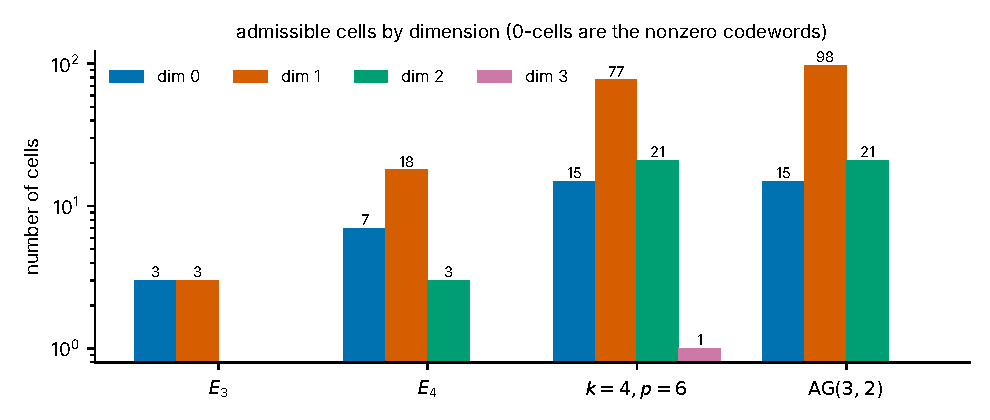
\includegraphics[width=0.95\textwidth]{figures/fig03_admissible_cells.pdf}
\caption{Numbers of cells of each dimension (dimension $0$ counts the nonzero codewords) for $E_3$, $E_4$, a minimal class with $k=4$, $p=6$, and $\AG(3,2)$. A cell is determined by a family $S$ of disjoint circuits and a coset of $\spn S$ (Lemma~\ref{lem:cellpair}). \figdesc{exact combinatorial data computed by \texttt{scripts/figs.py}; no higher-dimensional geometry is implied by the drawing.}}\label{fig:cells}
\end{figure}

\subsection{Collisions and embeddedness}

\begin{definition}[Collision; embedded]\label{def:collision}
Two \emph{distinct} cells $Z\ne Z'$ of positive dimension \emph{collide} if their relative interiors intersect; equivalently (Theorem~\ref{thm:centre}) if $U(S)=U(T)$ and $x=y$ off $U$. A collision is a pair $\{Z,Z'\}$ of colliding cells. The box is \emph{non-embedded} if it has a collision and \emph{embedded} otherwise.
\end{definition}

The word ``embedded'' is justified by the following description in terms of polyhedral complexes.

\begin{proposition}[Embedded $\Leftrightarrow$ face-to-face]\label{prop:facetoface}
The faces of a cell $Z(S,x)$ are the cells $Z(S',x')$ with $S'\subseteq S$ and $x'$ a vertex of $Z$, together with the vertices. The box is embedded if and only if any two cells (of any dimension) intersect in a common face, possibly empty; i.e.\ if and only if the cells form a polyhedral complex.
\end{proposition}

\begin{proof}
The cell is a product of segments, one per block, so its faces are the sub-products: choose a subfamily $S'\subseteq S$ to vary and fix every other block at one of its two endpoints; the result is $Z(S',x')$ with $x'$ a vertex (then $x'\notin\spn S'$, because $x'\oplus s'$ is a vertex of $Z$, hence nonzero, for every $s'\in\spn S'\subseteq\spn S$). If a collision $\{Z,Z'\}$ exists, the common centre lies in $Z\cap Z'$; if $Z\cap Z'$ were a face $G$ of both, then $G\ni\gamma$ with $\gamma\in\relint Z$ forces $G=Z$ (a face containing a point of the relative interior is the whole cell), and likewise $G=Z'$, so $Z=Z'$, a contradiction. Conversely suppose there is no collision, and let $Z,Z'$ be cells with $p\in Z\cap Z'$. The unique face $G$ of $Z$ with $p\in\relint G$ and the unique face $G'$ of $Z'$ with $p\in\relint G'$ are cells or vertices; if $G$ is a vertex then $p\in F$ is a $0/1$ point, and then $G'$ is also a vertex because the relative interior of a positive-dimensional cell contains no $0/1$ points (Lemma~\ref{lem:relint}); in the positive-dimensional case $\relint G\cap\relint G'\ne\emptyset$ and no collision forces $G=G'$. So every point of $Z\cap Z'$ lies in the relative interior of a common face. Taking $p$ to be the average of points chosen in the relative interiors of the common faces of maximal dimension, the minimal face of $Z$ containing $p$ is a common face containing all of them; hence $Z\cap Z'$ is a single common face.
\end{proof}

\subsection{Witnesses and ranks}

\begin{definition}[Witness; witness rank; $\rmin$]\label{def:witness}
Let $\{Z,Z'\}$ be a collision with generator matrices $A\,(r\times n)$ and $B\,(t\times n)$ and base points $x,y$; put $\delta=x-y$. The triple $(A,B,\delta)$ is a \emph{witness}. Its \emph{witness rank} is
\[
d_{\mathrm{span}}=\rk\begin{bmatrix}A\\ B\\ \delta\end{bmatrix}.
\]
The \emph{minimum witness rank} $\rmin(C)$ of a non-embedded box is the minimum of the witness rank over all collisions.
\end{definition}

\begin{lemma}[Witness rank is the dimension of the affine span]\label{lem:rankspan}
For a collision $\{Z,Z'\}$ the vector $\delta$ lies in the row space of $\begin{bmatrix}A\\B\end{bmatrix}$. Consequently the witness rank equals $\rk\begin{bmatrix}A\\B\end{bmatrix}$ and equals the dimension of the affine hull of $Z\cup Z'$. It is at least $\max(r,t)$ and at most $r+t$.
\end{lemma}

\begin{proof}
Let $\gamma$ be the common centre. Then $\gamma=x+\tfrac12\sum g_j=y+\tfrac12\sum h_l$ (rows $g_j$ of $A$, $h_l$ of $B$), so $\delta=x-y=\tfrac12\sum h_l-\tfrac12\sum g_j$. The affine hulls of $Z$ and $Z'$ are $\gamma+\mathrm{row}(A)$ and $\gamma+\mathrm{row}(B)$, so the hull of the union is $\gamma+\mathrm{row}(A)+\mathrm{row}(B)$. The rows of $A$ are independent (disjoint supports), similarly for $B$.
\end{proof}

\begin{remark}[Individual versus minimum]\label{rem:individual}
A collision may have witness rank larger than $3$; the quantity $\rmin$ takes the minimum. For instance the even-weight code $E_6$ (Section~\ref{sec:E4}) has $1710$ collisions: $720$ between cells of dimensions $(2,2)$ and $990$ between cells of dimensions $(3,3)$, with witness ranks $3,4,5,6$ occurring $585,360,585,180$ times (exact enumeration with the engine of Appendix~\ref{app:repro}), while the minimum is still $3$. Only the minimum is bounded.
\end{remark}

\begin{example}[An embedded box, $E_3$]\label{ex:E3}
Let $M=(1\,1\,1)$, $C=E_3=\{000,110,101,011\}$. The circuits are the three weight-two words, pairwise intersecting. A circuit family contains only one circuit, so all cells are $1$-dimensional: the cell of the circuit $c$ and base point $x\in C\setminus\{0,c\}$ joins the two remaining words (for $c=110$, $x=101$, the edge $101$--$011$). The fibre is a triangle with three edges, the cells form a complex, and the box is embedded; Theorem~\ref{thm:E1} below shows this without enumeration, since no set has two partitions.
\end{example}

\begin{figure}[ht]
\centering
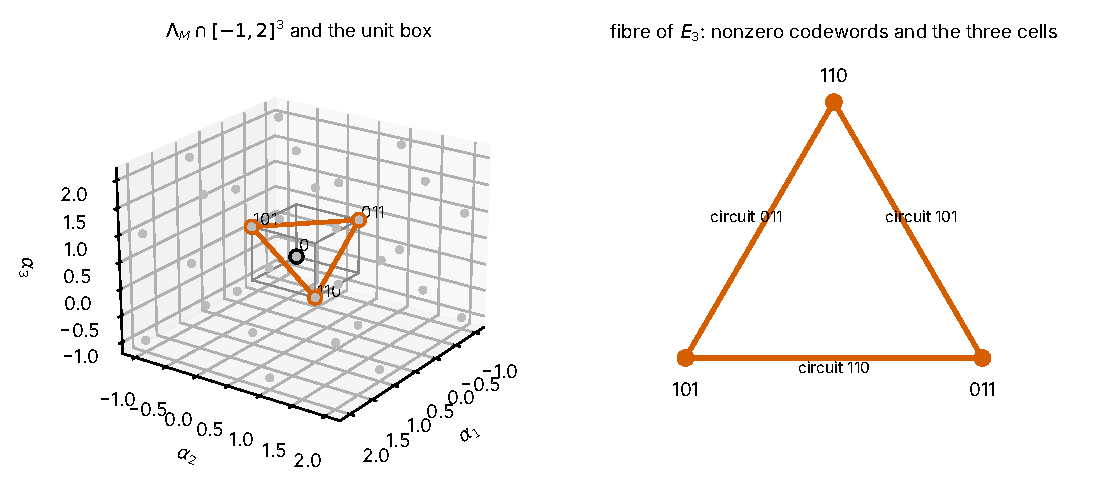
\includegraphics[width=0.92\textwidth]{figures/fig01_lattice_slice.pdf}
\caption{The binary relation lattice and its $0/1$ slice for $n=3$, $M=(1\,1\,1)$. Left: lattice points of $\Lambda_M$ in $\{-1,0,1,2\}^3$ (grey) and the unit box; the three nonzero fibre points $110,101,011$ are the vertices of the triangle (the edges are the three admissible cells). Right: the same data as codewords of $E_3$. \figdesc{exact integer coordinates generated by \texttt{scripts/figs.py}; a rendering of $n=3$ only, not of higher-dimensional geometry.}}\label{fig:lattice}
\end{figure}

\begin{figure}[ht]
\centering
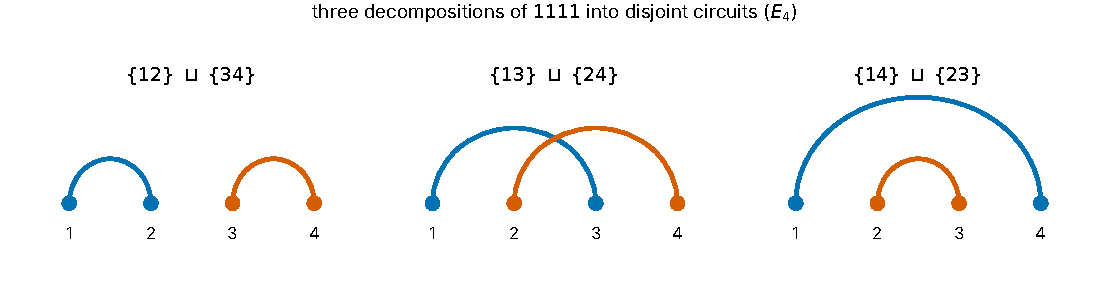
\includegraphics[width=0.92\textwidth]{figures/fig02_circuit_decompositions.pdf}
\caption{Circuits and decompositions in $E_4$. The word $1111$ has three distinct decompositions into pairs of disjoint circuits. \figdesc{generated by \texttt{scripts/figs.py} from the exact circuit list.}}\label{fig:decomp}
\end{figure}
